% Document Head
\documentclass[11pt, oneside]{book}
\usepackage{geometry}
\geometry{letterpaper}
\usepackage[parfill]{parskip}
\usepackage{graphicx}

% Essential Packages
\usepackage{ragged2e}
\usepackage{amssymb}
\usepackage{amsmath}
\usepackage{mathrsfs}
\usepackage[utf8]{inputenc}
\usepackage[english]{babel}
\usepackage{pgf,tikz}
\usepackage{pgfplots}
\usepackage[hyperref]{ntheorem}
\usepackage{hyperref}
\usepackage[noabbrev,capitalize,nameinlink]{cleveref}

% hyperref Package Settings
\usepackage{hyperref}
\hypersetup{
	colorlinks = true,
	linkcolor = magenta
}

% tikz Libraries
\usepgfplotslibrary{polar}
\usepgflibrary{shapes.geometric}
\usetikzlibrary{angles,patterns,calc}

% Theorem Style Customization
\setlength\theorempreskipamount{2ex}
\setlength\theorempostskipamount{3ex}

% ntheorem Declarations
\theoremstyle{break}
\newtheorem{thm}{Theorem}[section]
\newtheorem*{proof}{Proof}
\newtheorem*{solution}{Solution}
\newtheorem{crly}{Corollary}[section]
\newtheorem{lemma}{Lemma}[section]
\newtheorem{propo}{Proposition}[section]
\newtheorem*{remark}{Remark}
\newtheorem*{note}{Note}
\newtheorem*{notation}{Notation}
\newtheorem{ex}{Exercise}[section]
\newtheorem{defn}{Definition}[section]
\newtheorem{eg}{Example}[section]
\newtheorem{axiom}{Axiom}[section]

% ntheorem listtheorem style
\makeatother
\newlength\widesttheorem
\AtBeginDocument{
  \settowidth{\widesttheorem}{Proposition A.1.1.1\quad}
}

\makeatletter
\def\thm@@thmline@name#1#2#3#4{%
        \@dottedtocline{-2}{0em}{2.3em}%
                   {\makebox[\widesttheorem][l]{#1 \protect\numberline{#2}}#3}%
                   {#4}}
\@ifpackageloaded{hyperref}{
\def\thm@@thmline@name#1#2#3#4#5{%
    \ifx\#5\%
        \@dottedtocline{-2}{0em}{2.3em}%
            {\makebox[\widesttheorem][l]{#1 \protect\numberline{#2}}#3}%
            {#4}
    \else
        \ifHy@linktocpage\relax\relax
            \@dottedtocline{-2}{0em}{2.3em}%
                {\makebox[\widesttheorem][l]{#1 \protect\numberline{#2}}#3}%
                {\hyper@linkstart{link}{#5}{#4}\hyper@linkend}%
        \else
            \@dottedtocline{-2}{0em}{2.3em}%
                {\hyper@linkstart{link}{#5}%
                  {\makebox[\widesttheorem][l]{#1 \protect\numberline{#2}}#3}\hyper@linkend}%
                    {#4}%
        \fi
    \fi}
}

\makeatletter
\def\thm@@thmline@noname#1#2#3#4{%
        \@dottedtocline{-2}{0em}{5em}%
                   {{\protect\numberline{#2}}#3}%
                   {#4}}
\@ifpackageloaded{hyperref}{
\def\thm@@thmline@noname#1#2#3#4#5{%
    \ifx\#5\%
        \@dottedtocline{-2}{0em}{5em}%
            {{\protect\numberline{#2}}#3}%
            {#4}
    \else
        \ifHy@linktocpage\relax\relax
            \@dottedtocline{-2}{0em}{5em}%
                {{\protect\numberline{#2}}#3}%
                {\hyper@linkstart{link}{#5}{#4}\hyper@linkend}%
        \else
            \@dottedtocline{-2}{0em}{5em}%
                {\hyper@linkstart{link}{#5}%
                  {{\protect\numberline{#2}}#3}\hyper@linkend}%
                    {#4}%
        \fi
    \fi}
}

\theoremlisttype{allname}

% Custom math operator
% \DeclareMathOperator{\rem}{rem}
\DeclareMathOperator{\re}{Re}
\DeclareMathOperator{\im}{Im}
\DeclareMathOperator{\caparg}{Arg}

% Graph styles
\pgfplotsset{compat=1.15}
\usepgfplotslibrary{fillbetween}
\pgfplotsset{four quads/.append style={axis x line=middle, axis y line=
middle, xlabel={$x$}, ylabel={$y$}, axis equal }}
\pgfplotsset{four quad complex/.append style={axis x line=middle, axis y line=
middle, xlabel={$\re$}, ylabel={$\im$}, axis equal }}

% Shortcuts
\newcommand{\floor}[1]{\lfloor #1 \rfloor}      % simplifying the writing of a floor function
\newcommand{\ceiling}[1]{\lceil #1 \rceil}      % simplifying the writing of a ceiling function
\newcommand{\dotp}{\, \cdotp}			        % dot product to distinguish from \cdot
\newcommand{\qed}{\hfill\ensuremath{\square}}   % Q.E.D sign
\newcommand{\abs}[1]{\left|#1\right|}						% absolute value
\newcommand{\Arg}[1]{\caparg #1}
\renewcommand{\bar}[1]{\mkern 1.5mu \overline{\mkern -1.5mu #1 \mkern -1.5mu} \mkern 1.5mu}

% Main Body
\title{PMATH352W18 Complex Analysis - Class Notes}
\author{Johnson Ng}

\begin{document}
\hypersetup{pageanchor=false}
\maketitle
\hypersetup{pageanchor=true}
\tableofcontents

\chapter*{List of Definitions}
\theoremlisttype{all}
\listtheorems{defn}

\chapter*{List of Theorems}
\theoremlisttype{allname}
\listtheorems{axiom,lemma,thm,crly,propo}

\chapter{Lecture 1 - Jan 3, 2018}\label{chp:Lecture 1 - Jan 3, 2018}

\section{Complex Numbers and Their Properties}\label{sect:Complex Numbers and Their Properties}

\begin{defn}[Complex Number, Complex Plane]\label{defn:Complex Number, Complex Plane}
	A \textbf{complex number} is a vector in $\mathbb{R}^2$. The \textbf{complex plane}, denoted by $\mathbb{C}$, is a set of complex numbers,
	\begin{equation*}
		\mathbb{C} = \mathbb{R}^2 = \left\{ \begin{pmatrix} x \\ y \end{pmatrix} : x , y \in \mathbb{R} \right\}
	\end{equation*}
	In $\mathbb{C}$, we usually write \\
	\begin{center}
		\begin{tabular}{c c}
			$0 = \begin{pmatrix} 0 \\ 0 \end{pmatrix}$ & $1 = \begin{pmatrix} 1 \\ 0 \end{pmatrix}$ \\
			$i = \begin{pmatrix} 0 \\ 1 \end{pmatrix}$ & $x = \begin{pmatrix} x \\ 0 \end{pmatrix}$ \\
			$iy = \begin{pmatrix} 0 \\ y \end{pmatrix}$
		\end{tabular}
	\end{center}
	where $x, y \in \mathbb{R}$. Consequently, we have that
	\begin{equation*}
		x + iy = x + yi = \begin{pmatrix} x \\ y \end{pmatrix}
	\end{equation*}
	If for $x, y \in \mathbb{R}, \; z = x + iy$, then $x$ is aclled the real part of $z$ and $y$ is called the imaginary part of $z$, and we write
	\begin{equation*}
		\re(z) = x \quad \im(z) = y.
	\end{equation*}
\end{defn}

\begin{note}
	\begin{itemize}
		\item It is easy to see how $\mathbb{R}$ is a subset of $\mathbb{C}$.
		\item Complex Numbers of the form $\left(\begin{smallmatrix} 0 \\ y \end{smallmatrix}\right)$ where $y \in \mathbb{R}$ are called \textit{purely imaginary numbers}.
		\item Certain authors may prefer to denote $i = \left(\begin{smallmatrix} 0 \\ 1 \end{smallmatrix}\right)$.
	\end{itemize}
\end{note}

\begin{defn}[Sum and Product]\label{defn:Sum and Product}
	We define the sum of two complex numbers to be the usual vector sum, i.e.
	\begin{align*}
		(a + ib) + (c + id) &= \begin{pmatrix} a \\ b \end{pmatrix} + \begin{pmatrix} c \\ d \end{pmatrix} \\
											&= \begin{pmatrix} a + c \\ b + d \end{pmatrix} \\
											&= (a + c) + i (b + d)
	\end{align*}
	where $a, b, c, d \in \mathbb{R}$.

	We define the product of two complex numbers by setting $i^2 = -1$, and by requiring the product to be commutative, associative, and distributive over the sum. In this setup, we have that
	\begin{align}
		(a + ib)(c + id) &= ac + iad + ibc + i^2 bd \nonumber \\
						 &= (ac - bd) + i (ad + bc) \label{eq:complex multiplication}
	\end{align}
\end{defn}

\begin{note}
 It is interesting to note that \textit{any complex number times zero is zero}, just like what we have with real numbers.
 \begin{gather*}
 	\forall z = x + iy \in \mathbb{C} \; x, y \in \mathbb{R} \enspace 0 \in \mathbb{C} \\
 	z \cdot 0 = (x + iy)(0 + i0) = 0 + i0 = 0
 \end{gather*}
\end{note}

\begin{eg}\label{eg:1}
	Let $z = 2 + i, w = 1 + 3i$. Find $z + w$ and $zw$.
	\begin{align*}
		z + w &= (2 + i) + (1 + 3i) \\
			  	&= 3 + 4i \\
			  	\\
		zw 		&= (2 + i)(1 + 3i) \\
					&= (2 - 3) + i (6 + 1) \quad \text{By } \cref{eq:complex multiplication}\\
					&= -1 + 7i
	\end{align*}
\end{eg}

\begin{eg}\label{eg:multiplicative inverse of a complex number}
	Show that every non-zero complex number has a multiplicative inverse, $z^{-1}$, and find a formula for this inverse.

	Let $z = a + ib$ where $a, b \in \mathbb{R}$ with $a^2 + b^2 \neq 0$. Then
	\begin{align*}
				 & z(x + iy) = 1 \\
		\iff & (ax - by) + i(ay + bx) = 1 \\
		\iff & \begin{pmatrix} ax - by \\ ay + bx	\end{pmatrix} = \begin{pmatrix} 1 \\ 0 \end{pmatrix} \\
		\iff & \begin{pmatrix} a & -b \\ b & a \end{pmatrix}\begin{pmatrix} x \\ y \end{pmatrix} = \begin{pmatrix} 1 \\ 0 \end{pmatrix} \\
		\iff & \begin{pmatrix} x \\ y \end{pmatrix} = \frac{1}{a^2 + b^2} \begin{pmatrix} a & b \\ -b & a \end{pmatrix}	\begin{pmatrix} 1 \\ 0 \end{pmatrix} \\
		\iff & \begin{pmatrix} x \\ y \end{pmatrix} = \frac{1}{a^2 + b^2}\begin{pmatrix} a \\ -b \end{pmatrix} \\
		\iff & x + iy = \frac{a}{a^2 + b^2} - i \frac{b}{a^2 + b^2} 
	\end{align*}
	Therefore, we have that the formula for the inverse is
	\begin{equation}\label{eq:complex inverse}
		(a + ib)^{-1} = \frac{a}{a^2 +b^2} - i \frac{b}{a^2 + b^2} 
	\end{equation}
\end{eg}

\begin{notation}
	For $z, w \in \mathbb{C}$, we write
	\begin{center}
		\begin{tabular}{c c}
			$-z = -1z$ & $w - z = w + (-z)$ \\
			$\frac{1}{z} = z^{-1}$ & $\frac{w}{z} = wz^{-1}$
		\end{tabular}
	\end{center}
\end{notation}

\begin{eg}\label{eg:3}
	Find $\frac{(4 - i) - (1 - 2i)}{1 + 2i}$.
	\begin{align*}
		\frac{(4 - i) - (1 - 2i)}{1 + 2i} &= \frac{3 + i}{1 + 2i} \\
					&= (3 + i)(\frac{1}{5} - i \frac{2}{5} ) \\
					&= 1 - i
	\end{align*}
\end{eg}

\begin{note}
	The set of complex numbers is a \textbf{field} under the operations of additiona and multiplication. This means that $\forall u, v, w \in \mathbb{C}$,
	\begin{center}
		\begin{tabular}{r@{\;{=}\;}l r@{\;{=}\;}l}
			u + v 			& v + u 			& uv 			& vu \\
			(u + v) + w & u + (v + w) & (uv)w 	& u(vw) \\
			0 + u 			& u 					& 1u			& u \\
			u + (-u)		& 0						& $uu^{-1}$	& 1, $\; u \neq 0$ \\
			u(v + w)		& uv + uw
		\end{tabular}
	\end{center}

	Since the distributive law holds for complex numbers, note that the binomial expansion works for $(w + z)^n$ where $w, z \in \mathbb{C}$ and $n \in \mathbb{N}$. (I did not verify if this is still true for when $n \in \mathbb{R}$.)
\end{note}

\begin{defn}[Conjugate]\label{defn:Conjugate}
	If $z = x + iy$ where $x, y \in \mathbb{R}$, then the $\textbf{conjugate of z}$ is given by $\bar{z} = x - iy$
\end{defn}

\begin{eg}\label{eg:4}
	Let $z = 3 + 4i$. Then the $\bar{z} = 3 - 4i$. Represented in the complex plane, we have the following:
	\begin{center}
		\begin{tikzpicture}
			\begin{axis}[four quad complex, xtick={-4,-3,...,4}, ytick={-5,-4,...,5}, xmin=-4, xmax=4, ymin=-5, ymax=5]
				\node[label={0:{$z$}},circle,fill,inner sep=2pt] at (axis cs:3,4) {};
				\node[label={0:{$\bar{z}$}},circle,fill,inner sep=2pt] at (axis cs:3,-4) {};
			\end{axis}
		\end{tikzpicture}
	\end{center}

	We observe that on the complex plane, the conjugate of a complex number is simply its reflection on the real axis.
\end{eg}

\begin{defn}[Modulus]\label{defn:Modulus}
	We define the \textbf{modulus} (length, magnitude) of $z = x + iy \in \mathbb{C}, x, y \in \mathbb{R}$, to be
	\begin{equation}
		\abs{z} = \sqrt{x^2 + y^2} \in \mathbb{R}.
	\end{equation}
\end{defn}

\begin{note}
 Note that this definition is consistent with the notion of the absolute value in real numbers when $z$ is a real number, since if $y = 0$, $\abs{z} = \abs{x + i0} = \sqrt{x^2} = \pm x$.
\end{note}

\begin{note}
 For $z, w \in \mathbb{R}$, we have
 \begin{center}
 	\begin{tabular}{r@{\;{=}\;}l r@{\;{=}\;}l r@{\;{=}\;}l}
 		$\bar{\bar{z}}$ 	& z 									& $z + \bar{z}$ 	& $2 \re(z)$ 			& $z - \bar{z}$ 	& $2i \im(z)$ \\
 		$z\bar{z}$				& $\abs{z}^2$					& $\abs{z}$				& $\abs{\bar{z}}$	& $\bar{z \pm w}$	& $\bar{z} \pm \bar{w}$ \\
 		$\bar{zw}$		& $\bar{z} - \bar{w}$	& $\abs{zw}$			&	$\abs{z}\abs{w}$
 	\end{tabular}
 \end{center}
 but note that $\abs{z + w} \neq \abs{z} + \abs{w}$.
\end{note}

\begin{note}
 While inequalities such as $z_1 < z_2$, where $z_1, z_2 \in \mathbb{C}$, are meaningless unless if both of them are real, $\abs{z_1} < \abs{z_2}$ means that the point $z_1$ in the complex plane is closer to the origin than the point $z_2$.
\end{note}

\begin{propo}[Basic Inequalities]\label{propo:Basic Inequalities}
	\begin{enumerate}
		\item $\abs{\re(z)} \leq \abs{z}$ \\
		\item $\abs{\im(z)} \leq \abs{z}$ \\
		\item $\abs{z + w} \leq \abs{z} + \abs{w} \quad$ Triangle Inequality \label{eq:triangle inequality}\\
		\item $\abs{z + w} \geq \abs{\;\abs{z} - \abs{w}\;} \quad$ Inverse Triangle Inequality
	\end{enumerate}
\end{propo}

\begin{proof}
	Note that $\abs{z}^2 = \re(z)^2 + \im(z)^2$ and that we can express $\abs{x} = \sqrt{x^2}$ for any $x \in \mathbb{R} $. 1 and 2 immediately follows from that.

	To prove 3, we have that
	\begin{align*}
		\abs{z + w}^2 &= (z + w)(\bar{z} + \bar{w}) \\
									&= \abs{z}^2 + \abs{w}^2 + (w\bar{z} + \bar{w}z) \\
									&= \abs{z}^2 + \abs{w}^2 + 2\re(w\bar{z}) \\
									&\leq \abs{z}^2 + \abs{w}^2 + 2\abs{w\bar{z}} \quad \text{by 1} \\
									&= \abs{z}^2 + \abs{w}^2 + 2\abs{wz} \quad \text{since } \abs{w\bar{z}} = \abs{w}\abs{\bar{z}} \text{ and } \abs{z} = \abs{\bar{z}} \\
									&= (\abs{z} + \abs{w})^2
	\end{align*}
	
	To prove 4, note that
	\begin{alignat}{3}
		&\abs{z} &&= \abs{z + w - w} &&\leq \abs{z + w} + \abs{w} \label{basicinequal1} \\
		&\abs{w} &&= \abs{w + z - z} &&\leq \abs{z + w} + \abs{z} \label{basicinequal2}
	\end{alignat}

	Observe that
	\begin{align*}
		\cref{basicinequal1} \implies \abs{z} - \abs{w} \leq \abs{z + w} \\
		\cref{basicinequal2} \implies \abs{w} - \abs{z} \leq \abs{z + w}
	\end{align*}

	Thus, we have that
	\begin{equation*}
		\abs{z + w} \geq \abs{\; \abs{z} - \abs{w} \;}
	\end{equation*}
	as required.\qed
\end{proof}

\cref{eq:triangle inequality} in \cref{propo:Basic Inequalities} can be generalized by the means of mathematical induction to sums involving any finite number of terms, as:
\begin{equation}\label{eq:generalized triangle inequality}
	\abs{z_1 + z_2 + \hdots + z_n} \leq \abs{z_1} + \abs{z_2} + \hdots + \abs{z_n}
\end{equation}
where $n \in \mathbb{N} \setminus \{0, 1\}$.

To note the induction proof, when $n = 2$, \cref{eq:generalized triangle inequality} is just \cref{eq:triangle inequality}. If \cref{eq:generalized triangle inequality} is true for when $n = m$ where $m \in \mathbb{N} \setminus \{0, 1\}$, $n = m + 1$ is also true since by \cref{eq:triangle inequality},
\begin{align*}
	\abs{(z_1 + z_2 + \hdots + z_m) + z_{m+1}} &\leq \abs{z_1 + z_2 + \hdots + z_m} + \abs{z_{m + 1}} \\
			&\leq (\abs{z_1} + \abs{z_2} + \hdots + \abs{z_m}) + \abs{z_{m+1}}.
\end{align*}

The distance between two points $z_1 = x_1 + iy_1, z_2 = x_2 + iy_2 \in \mathbb{C}, x_1, x_2, y_1, y_2 \in \mathbb{R}$ is $\abs{z_1 - z_2}$, since $\abs{z_1 - z_2} = \sqrt{(x_1 - x_2)^2 (y_1 - y_2)^2}$ is our usual notion of the Euclidean distance of two points on a plane.

Also, note that
\begin{equation*}
	z_1 - z_2 = z_1 + (-z_2)
\end{equation*}
and thus if we apply our knowledge of vector representation, $z_1 - z_2$ is the directed line segment from the point $z_2$ to $z_1$.

With the notion of a ``distance'' set on the complex plane, we can now explore upon points lying on a circle with a center $z_0$ and radius $R$, which satisfies the equation
\begin{equation*}
	\abs{z - z_0} = R.
\end{equation*}
We may simply refer to this set of points as the circle $\abs{z - z_0} = R$.

\begin{eg}
	We may describe a set $\left\{z \in \mathbb{C} : \abs{z -i} = 1 \right\}$ as follows:

	\begin{center}
		\begin{tikzpicture}
			\begin{axis}[four quad complex, xtick={-3,-2,...,3}, ytick={-3,-2,...,3}, xmin=-3, xmax=3, ymin=-1, ymax=3]
				\draw (axis cs:0, 1) circle [radius=1];
			\end{axis}
		\end{tikzpicture}
	\end{center}

	Let $a, b \in \mathbb{C}$ describe the set $\left\{z \in \mathbb{C} : \abs{z - a} < \abs{z - b} \right\}$.

	Suppose the following coordinates for $a$ and $b$ are arbitrary,

	\begin{center}
		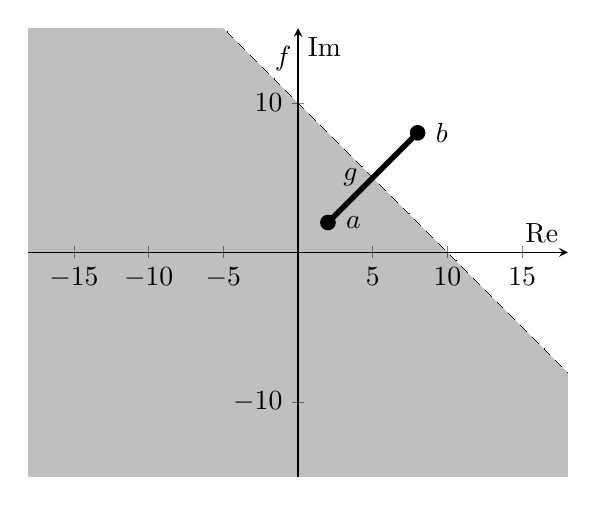
\begin{tikzpicture}
			\begin{axis}[four quad complex, xmin=-15, xmax=15, ymin=-15, ymax=15]
				\draw[line width=0pt,dashed,fill=black,fill opacity=0.25](-20,20)--(-20,-20)--(20,-20)--(20,-10)--(-5,15);
				\draw[color=black] (-1,13) node {$f$};
				\draw[line width=2pt,solid](2,2)--(8,8);
				\draw[color=black] (3.5,5) node {$g$};
				\node[label={0:{$a$}},circle,fill,inner sep=2pt] at (axis cs:2,2) {};
				\node[label={0:{$b$}},circle,fill,inner sep=2pt] at (axis cs:8,8) {};
			\end{axis}
		\end{tikzpicture}
	\end{center}

	In the above, $g$ is the line segment that connects the points $a$ and $b$ on the complex plane, while $f$ is the perpendicular bisector of the line segment $g$. The area described by the set $\left\{z \in \mathbb{C} : \abs{z - a} < \abs{z - b} \right\}$ is the shaded area which is below $f$.
\end{eg}

\chapter{Lecture 2 - Jan 5th, 2018}\label{chp:Lecture 2 - Jan 5th, 2018}

\section{Complex Numbers and Their Properties (Continued)}\label{sect:Complex Numbers and Their Properties (Continued)}

\begin{eg}
	Let $a \in \mathbb{C}$. Describe the set $\{z \in \mathbb{C} : 1 < \abs{z-a} < 2\}$.

	\begin{center}
		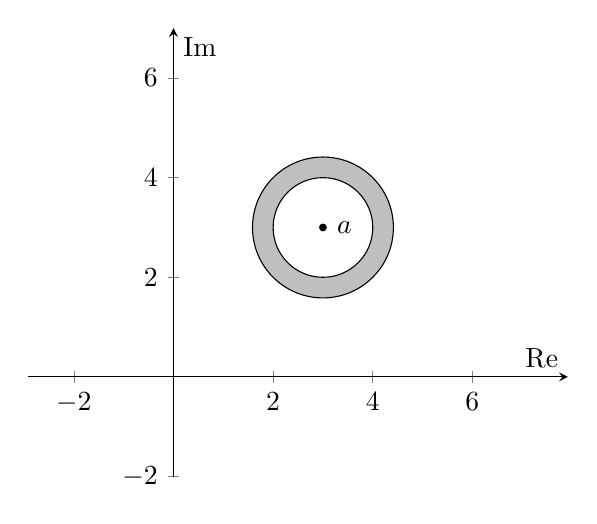
\begin{tikzpicture}
			\begin{axis}[
				four quad complex,
				xmin=-2, xmax=7,
				ymin=-2, ymax=7
			]
				\draw [fill=black,fill opacity=0.25] (3,3) circle (1.4142135623730951);
				\draw[fill=white](3,3) circle (1);
				\node[label={0:{$a$}},circle,fill,inner sep=1pt] at (axis cs:3,3) {};
			\end{axis}
		\end{tikzpicture}
	\end{center}
\end{eg}

\begin{eg}
	\label{eg:complex number has exactly two roots}
	Show that every non-zero complex number has exactly two complex square roots, and find a formula for the square roots.

	Let $z = x + iy \in \mathbb{C}, x, y \in \mathbb{R}$, and let $w = u + iv, u, v \in \mathbb{R}$. Then

	\begin{alignat}{3}
		&w^2 = z &&\iff && (u + iv)^2 = x + iy \nonumber \\
		&	&&\iff 	&& (u^2 - v^2) + i(2uv) = x + iy \nonumber \\
		&	&&\iff && x = u^2 + v^2 \quad \text{and} \label{tworoots 1} \\
		&	&&	   && y = 2uv \label{tworoots 2}
	\end{alignat}

	Square both sides of \cref{tworoots 2}, and thus we have $y^2 = 4u^2 v^2$.

	Multiply \cref{tworoots 1} by $4u^2$, and we get
	\begin{alignat*}{3}
		& 	  &&4u^2 x &&= 4u^4 - 4u^2 v^2 = 4u^4 - y^2 \\
		&\iff &&0 	&&= 4u^4 - 4u^2 x - y^2 \\
		&\iff &&u^2 &&= \frac{4x \pm \sqrt{16x^2 + 16y^2}}{8} \\
		&	  &&	&&= \frac{x \pm \sqrt{x^2 + y^2}}{2} 
	\end{alignat*}

	Suppose $y \neq 0$. Note that $x < \sqrt{x^2 + y^2}$. Thus $u^2 = \frac{x + \sqrt{x^2 + y^2}}{2} \implies u = \left(\frac{x + \sqrt{x^2 + y^2}}{2} \right)^{\frac{1}{2}}$.

	Similarly, we can get
	\begin{equation*}
		v = \pm \left(\frac{-x + \sqrt{x^2 + y^2}}{2}\right)^{\frac{1}{2}}
	\end{equation*}

	Note that all four choices of signs satisfy \cref{tworoots 1}. If $y > 0$, then $u$ and $v$ are either both positive or both negative by \cref{tworoots 2}.

	Suppose $y = 0$. Then we have
	\begin{equation*}
		w^2 = z = x
	\end{equation*}

	Therefore, we get
	\begin{equation*}
		w = \begin{cases}
			\pm \left[ \left(\frac{x + \sqrt{x^2 + y^2}}{2} \right)^{\frac{1}{2}} + i \left( \frac{-x + \sqrt{x^2 + y^2}}{2} \right)^{\frac{1}{2}} \right] & y > 0 \\
			\pm \left[ \left(\frac{x + \sqrt{x^2 + y^2}}{2} \right)^{\frac{1}{2}} - i \left(\frac{-x + \sqrt{x^2 + y^2}}{2} \right)^{\frac{1}{2}} \right] & y < 0 \\
			\pm \sqrt{x} & y = 0, x > 0 \\
			\pm i \sqrt{x} & y = 0, x < 0
		\end{cases}
	\end{equation*}
\end{eg}

\begin{remark}
	Let $z \in \mathbb{C}$. The notation $\sqrt{z}$ may represent either one of the square roots of $z$ or both of the square roots, i.e. it is possible that $\sqrt{z}$ represents a set.
\end{remark}

\begin{ex}\label{ex:Separation of Multiplication in Square Roots}
	Is it always okay for complex numbers such that $\sqrt{zw} = \sqrt{z} \sqrt{w}$, for $z, w \in \mathbb{C}$?

	No. For example, consider $z = w = -1$. Then we have
	\begin{equation*}
		\sqrt{zw} = \sqrt{1} = \pm 1
	\end{equation*}
	while
	\begin{equation*}
		\sqrt{z} \sqrt{w} = i \cdot i = -1
	\end{equation*}
	and thus
	\begin{equation*}
		\sqrt{zw} \neq \sqrt{z} \sqrt{w}.
	\end{equation*}
\end{ex}

\begin{eg}
	Find the values of $\sqrt{3 - 4i}$.

	By \cref{eg:complex number has exactly two roots},

	\begin{align*}
		\sqrt{3 - 4i} &= \pm \left( \sqrt{\frac{3 + \sqrt{9 + 16}}{2}} - i \sqrt{\frac{-3 + \sqrt{9 + 16}}{2}} \right) \\
			&= \pm (2 - i)
	\end{align*}
\end{eg}

\begin{remark}\label{remark:quadratic formula for complex numbers}
	The quadratic formula holds for complex polynomials, i.e.
	\begin{equation*}
		\forall a, b, c \in \mathbb{C} \quad a \neq 0 \quad \forall z \in \mathbb{C} \; az^2 + bz + c = 0,
	\end{equation*}
	the solution for $z$ is given by
	\begin{equation}\label{eq:quadractic formula for complex numbers}
		z_{1, 2} = \frac{-b + \sqrt{b^2 - 4ac}}{b} 
	\end{equation}

	The following is a short proof.

	\begin{proof}
		\begin{align*}
			az^2 + bz + c = 0 &\iff z^2 + \frac{b}{a} z + \frac{c}{a} = 0 \\
				&\iff z^2 + \frac{b}{a} z + \left(\frac{b}{2a} \right)^2 - \left(\frac{b}{2a}\right)^2 + \frac{c}{a} = 0 \\
				&\iff \left(z + \frac{b}{2a} \right)^2 = \frac{b^2}{4a^2} - \frac{c}{a} = \frac{b^2 - 4ac}{4a^2} \\
				&\iff z = \frac{-b + \sqrt{b^2 - 4ac}}{2a}  
		\end{align*}
	\end{proof}

	(Personal Note: where did the $-$ for the supposed $\pm$ go? Or should it really be $\pm$?)
\end{remark}

\begin{eg}
	Solve $iz^2 - (2 + 3i)z + 5(1 + i) = 0$.
	\begin{align*}
		z &= \frac{2 + 3i + \sqrt{(2 + 3i)^2 - 4i[5(1 + i)]}}{2i} \\
			&= \frac{2 + 3i + \sqrt{-5 + 12i -20i + 20}}{2i} \\
			&= \frac{2 + 3i + \sqrt{15 + 8i}}{2i} 
	\end{align*}
	Note that by \cref{eg:complex number has exactly two roots},
	\begin{align*}
		\sqrt{15 - 8i} &= \pm \left[ \sqrt{\frac{15 + \sqrt{225 + 64}}{2} } - i \sqrt{\frac{-15 + \sqrt{225 + 64}}{2} } \; \right] \\
			&= \pm \left[ \sqrt{\frac{15 + 17}{2} } - i \sqrt{\frac{-15 + 17}{2} } \; \right] \\
			&= \pm (4 - i)
	\end{align*}
	Thus we have
	\begin{align*}
		z &= \frac{2 + 3i + \sqrt{15 + 8i}}{2i} \\
			&= \frac{2 + 3i \pm (4 - i)}{2i} \\
			&= (6 + 2i) \left( -\frac{1}{2}i \right) \text{ or } (-2 + 4i) \left( -\frac{1}{2} i \right) \quad \text{by } \cref{eg:multiplicative inverse of a complex number} \\
			&= (1 - 3i) \text{ or } (2 + i)
	\end{align*}
\end{eg}

\chapter{Lecture 3 - Jan 8th, 2018}\label{chp:Lecture 3 - Jan 8th, 2018}

\section{Complex Numbers and Their Properties (Continued 2)}\label{sect:Complex Numbers and Their Properties (Continued 2)}

\begin{defn}[Argument of a Complex Number]\label{defn:Argument of a Complex Number}
	Let $z \in \mathbb{C} \setminus \{0\}$. The \textbf{argument} (or the angle) of $z$, denoted by $\arg{z}$, $\Arg{z}$, or simply $\theta = \theta(z)$, is the angle modulo $2 \pi$ (i.e. $0 \leq \theta < 2 \pi$) between the vector defining $z$ and the positive real axis (in the counterclockwise direction).

	\begin{center}
		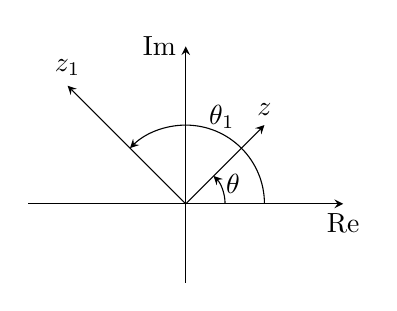
\begin{tikzpicture}
			\tikzset{>=stealth}
			\draw[->] (-2, 0) -- ++(4, 0) coordinate (X) node[below] {$\re$};
			\draw[->] (0, -1) -- ++(0, 3) node[left] {$\im$};
			\coordinate (O) at (0, 0);

			\draw[->] (O) -- (1,1) coordinate (z) node[above] {$z$};
			\path (X) -- (O) -- (z) pic [draw,->,pic text=$\theta$, angle eccentricity=1.3] {angle=X--O--z};

			\draw[->] (O) -- (-1.5, 1.5) coordinate (z1) node[above] {$z_1$};
			\path (X) -- (O) -- (z1) pic [draw,->,angle radius=1cm, pic text=$\theta_1$, angle eccentricity=1.2] {angle=X--O--z1};
		\end{tikzpicture}
	\end{center}
\end{defn}

\begin{notation}
	Let $e^{i \theta} := \cos \theta + i \sin \theta$. Note that this definition can be derived by the extending the Taylor expansion of $e^x = \sum_{n=0}^{\infty} \frac{x^n}{n!} $ for when $x \in \mathbb{C}$ (the sum of the real parts of the expansion is the Taylor expansion of cosine while the imaginary part for sine).

	Now $e^{i \theta}$ is on the unit circle.
	\begin{center}
		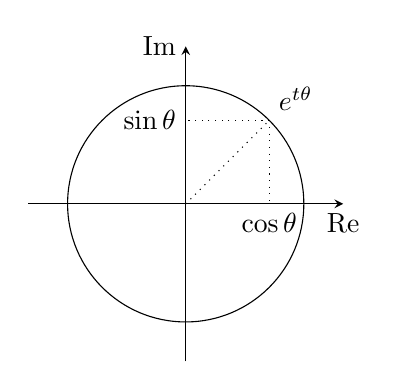
\begin{tikzpicture}
			\tikzset{>=stealth}
			\draw[->] (-2, 0) -- ++(4, 0) coordinate (X) node[below] {$\re$};
			\draw[->] (0, -2) -- ++(0, 4) node[left] {$\im$};
			\coordinate (O) at (0, 0);

			\newcommand \CircleRadius{1.5};
			\draw (0,0) circle (\CircleRadius);
			\coordinate (z) at (45:\CircleRadius);

			\draw[dotted] (O) -- (z) node[above right] {$e^{t \theta}$};
			\draw[dotted] (z) -- (z -| O) node[left] {$\sin \theta$};
			\draw[dotted] (z) -- (z |- O) node[below] {$\cos \theta$};
		\end{tikzpicture}
	\end{center}
\end{notation}

\begin{eg}
Some examples of $\theta \in [0, 2\pi)$:

	\begin{tabular}{r@{\;{=}\;}l r@{\;{=}\;}l}
		$e^{i \frac{\pi}{4}}$ & $\frac{\sqrt{2}}{2} + i \frac{\sqrt{2}}{2}$ & $e^{i \frac{\pi}{2} }$ & $i$ \\
		$e^{i \frac{3 \pi}{4}}$ & $-\frac{\sqrt{2}}{2} + i \frac{\sqrt{2}}{2}$ & $e^{i \pi} + 1$ & $0$
	\end{tabular}
\end{eg}

\begin{remark}
	\begin{equation*}
		\forall k \in \mathbb{Z} \enspace \forall \theta \in \mathbb{R} \enspace e^{i\theta} = e^{i(\theta + 2\pi k)} 
	\end{equation*}
\end{remark}

\begin{remark}
	The complex number $re^{i \theta}$, where $r > 0, \theta \in [0, 2\pi)$, represents the complex number with modulus $r$ and argument $\theta$.
	\begin{center}
		\begin{tikzpicture}
			\tikzset{>=stealth}
			\draw[->] (-2, 0) -- ++(4, 0) coordinate (X) node[below] {$\re$};
			\draw[->] (0, -2) -- ++(0, 4) node[left] {$\im$};
			\coordinate (O) at (0, 0);

			\newcommand \CircleRadius{1.5};
			\draw[dotted] (0,0) circle (\CircleRadius);
			\coordinate (z) at (135:\CircleRadius);

			\draw[<->] (O) -- (z) node[midway,below] {$r$} node[above left] {$z$};
			\path (X) -- (O) -- (z) pic [draw,->,angle radius=0.5cm,pic text=$\theta$,angle eccentricity=1.3] {angle=X--O--z};
		\end{tikzpicture}
	\end{center}

	Therefore, $\forall z \in \mathbb{C}$, we can express
	\begin{equation}\label{eq:polar representation of a complex number}
		z := \abs{z} e^{i \Arg{z}}.
	\end{equation}
\end{remark}

With that, we now have two representations of a complex number:
\begin{itemize}
	\item Cartesian representation: $z = x + iy$ where $x = \re(z)$ and $y = \im(z)$
	\item Polar representation: $z = re^{i \theta}$ where $r = \abs{z}$ and $\theta = \Arg{z} \in [0, 2\pi)$
\end{itemize}

To convert between the two representations, we have the following equations:

Polar $\to$ Cartesian:

\begin{equation}\label{eq:polar to cartesian}
	x = r \cos \theta \quad y = r \sin \theta
\end{equation}

Cartesian $\to$ Polar:

\begin{gather}\label{eq:cartesian to polar}
	r = \abs{z} \nonumber \\
	x \neq 0 \implies \tan \theta = \frac{y}{x} \\
	x = 0 \implies \theta = \frac{\pi}{2} \text{ or } \frac{3\pi}{2} \nonumber
\end{gather}

On another note,
\begin{equation*}
	z = re^{i \theta} \implies \bar{z} = re^{-i \theta}
\end{equation*}
and
\begin{equation*}
	z \neq 0 \implies \frac{1}{z} = \frac{1}{r} e^{-i \theta}
\end{equation*}

\begin{remark}
	\begin{gather*}
		\forall r_1, r_2 \in \mathbb{R} \; \forall \theta_1, \theta_2 \in [0, 2\pi) \\
		z_1 := r_1 e^{i \theta_1} \quad z_2 := r_2 e^{i \theta_2}
	\end{gather*}
	Then
	\begin{equation*}
		z_1 z_2 = r_1 r_2 e^{i \theta_1} e^{i \theta_2} = r_1 r_2 e^{i (\theta_1 + \theta_2)}
	\end{equation*}

	Note that $e^{ix} e^{iy} = e^{i(x + y)}$ is true for all $x, y \in \mathbb{R} $ since
	\begin{align*}
		e^{ix} e^{iy}
			&= (\cos x + i \sin x)(\cos y + i \sin y) \\
			&= (\cos x \cos y - \sin x \sin y) + i (\cos x \sin y + \cos y \sin x) \\
			&= \cos (x + y) + i \sin (x + y) \\
			&= e^{i (x + y)}.
	\end{align*}

	Generalizing the above, we get that
	\begin{equation*}
		\forall n \in \mathbb{Z} \enspace (re^{in}) = r^n e^{in\theta}
	\end{equation*}
	which is commonly known as \textbf{deMoivre's Law}.
\end{remark}

\begin{propo}[nth Roots of a Complex Number]\label{propo:nth Roots of a Complex Number}
	\begin{gather*}
		\forall z = re^{i\theta} \in \mathbb{C} \enspace r = \abs{z} \in \mathbb{R} \enspace \theta \in [0, 2\pi) \\
		\exists w = se^{i\tau} \in \mathbb{C} \enspace s \in \mathbb{R} \enspace \tau \in [0, 2\pi) \\
		\forall n \in \mathbb{Z} \\ 
		w^n = \left( se^{i\tau}\right)^n = z = re^{i\theta}
	\end{gather*}

	The nth roots of $z$ is described by the set
	\begin{equation}\label{eq:nth roots of a complex number}
		\left\{ r^{\frac{1}{n}} e^{i \left(\frac{\theta + 2 \pi k}{n} \right)} : k = 0, 1, ..., n - 1 \right\}
	\end{equation}

	\begin{proof}
		\begin{gather*}
			s^n = r \iff s = r^{\frac{1}{n}} \\
			e^{in\theta} = e^{i \tau} \iff \theta = \frac{\tau + 2 \pi k}{n}
		\end{gather*}

		Therefore, the set that describes the nth roots of $z$ is
		\begin{gather*}
			\left\{ w = r^\frac{1}{n} e^{i \left( \frac{\theta + 2 \pi k}{n} \right)} : k = 0, 1, ..., n - 1 \right\}
		\end{gather*}
	\end{proof}
\end{propo}

\begin{remark}[nth Roots of Unity]\label{remark:nth Roots of Unity}
	The nth roots of unity is a direct consequence of \cref{propo:nth Roots of a Complex Number} where we solve for the equation $z^n = 1$ for any $z \in \mathbb{C}, n \in \mathbb{Z}$.

	The set that describes the nth roots of unity is
	\begin{equation}\label{eq:nth roots of unity}
		\left\{ e^{i \theta} : \theta = \frac{2 \pi k}{n}, k = 0, 1, ..., n - 1 \right\}
	\end{equation}
\end{remark}

It is easy to see how the nth roots of unity partitions the unit circle into n parts.

\begin{eg}
	Find the cubic roots of $-2 + 2i$.

	Let $z = -2 + 2i$. Note that $\abs{z} = 2\sqrt{2}$ and $\Arg{z} = \frac{3 \pi }{4}$.

	Therefore, in polar form, $z = 2 \sqrt{2} e^{i \frac{3\pi}{4} }$.

	Let $w = re^{i \theta}$, where $\theta \in [0, 2\pi)$, and $w^3 = z$. Then
	\begin{gather*}
		r = (2 \sqrt{2})^\frac{1}{3} \\
		\theta = \frac{\frac{3\pi}{4} + 2 \pi k}{3}, \enspace k = 0, 1, 2
	\end{gather*}

	The set that describes the cubic root of $-2 + 2i$ is thus
	\begin{equation*}
		\left\{ (2\sqrt{2})^\frac{1}{3} e^{i \theta} : \theta = \frac{\frac{3\pi}{4} + 2 \pi k}{3}, k = 0, 1, 2 \right\}
	\end{equation*}
\end{eg}

\begin{eg}
	Describe the set $\{z \in \mathbb{C} : \abs{\Arg{z} - \frac{\pi}{2}} < \frac{\pi}{2} \}$. (Note: $\Arg{z} \in [0, 2\pi)$)

	\begin{center}
		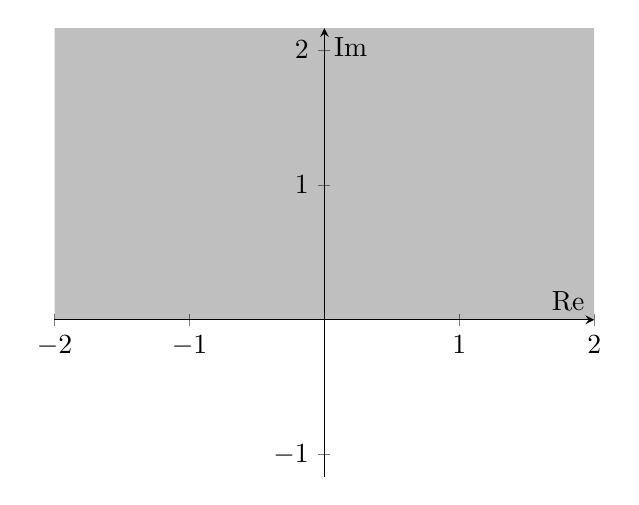
\begin{tikzpicture}
			\begin{axis}[four quad complex, xmin=-2, xmax=2, ymin=-1, ymax=2]
				\draw[line width=0pt,dashed,fill=black,fill opacity=0.25](-3,0)--(3,0)--(3,3)--(-3,3);
			\end{axis}
		\end{tikzpicture}
	\end{center}
\end{eg}

\begin{ex}
	Solve
	\begin{enumerate}
		\item $z^4 = -1$
			\begin{gather*}
				\text{Let } z = re^{i \theta} \\
				r = \abs{-1} = 1 \quad \theta = \frac{\pi + 2 \pi k}{4} = \frac{(2k + 1) \pi}{4}, \enspace k = 0, 1, 2, 3
			\end{gather*}
		\item $z^4 = -1 + \sqrt{3} i$
			\begin{gather*}
				\text{Let } z = re^{i \theta} \\
				r = \abs{-1 + \sqrt{3} i} = \sqrt{(-1)^2 + 3^2} = \sqrt{10} \\
				\theta = \frac{\frac{2\pi}{3} + 2\pi k}{4} = \frac{(2k + \frac{2}{3}) \pi}{4}, \quad k = 0, 1, 2, 3  
			\end{gather*}
	\end{enumerate}
\end{ex}

\chapter{Lecture 4 - Jan 10th, 2018}\label{chp:Lecture 4 - Jan 10th, 2018}

\section{Examples for nth Roots of Unity}\label{sect:Examples for nth Roots of Unity}

Recall that the $n$th roots of unity are given by $e^{i \frac{2\pi k}{n}}, k = 0, 1, ..., n - 1$.

\begin{ex}\label{ex:sum of root of unity other than one is negative one}
	Let $z$ be any $n$th root of unity other than 1. Show that
	\begin{equation}
		z^{n - 1} + z^{n - 2} + \hdots + z + 1 = 0
	\end{equation}

	\begin{proof}
		By the Sum of Finite Geometric Terms,
		\begin{equation*}
			z^{n - 1} + z^{n - 2} + \hdots + z + 1 = \frac{1 - z^n}{1 - z}.
		\end{equation*}
		Since $z^n = 1$, RHS is thus zero, which in turn completes the proof.
	\end{proof}
\end{ex}

As an aside, if we wish to remove the restriction that $z$ can also be 1, we may consider that
\begin{equation*}
	z^n - 1 = (z - 1)(1 + z + \hdots + z^{n - 1})
\end{equation*}
Since $z^n = 1$, LHS is zero. Then either $z = 1$ or $(1 + z + \hdots + z^{n - 1}) = 0$.

\begin{ex}
	Consider the $n - 1$ diagonals of a regular $n$-gon, inscribed in a circle of radius 1, obtained by connecting one vertex on the $n$-gon to all its other vertices.

	For example, if we are given $n = 6$, we obtain the following diagram.

	\begin{figure}
		\begin{center}
			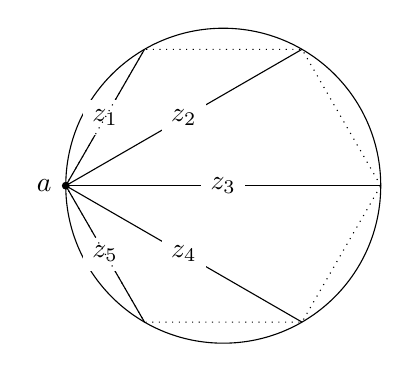
\begin{tikzpicture}
				\newcommand \CircleRadius {2};
				\draw(0, 0) circle (\CircleRadius);
				\coordinate (a) at (180:\CircleRadius);
				\coordinate (z1) at (120:\CircleRadius);
				\coordinate (z2) at (60:\CircleRadius);
				\coordinate (z3) at (0:\CircleRadius);
				\coordinate (z4) at (300:\CircleRadius);
				\coordinate (z5) at (240:\CircleRadius);
				\node[label={180:{$a$}},circle,fill,inner sep=1pt] at (a) {};
				\foreach \x in {1, ..., 5} {
					\draw (a)--(z\x) node[midway,fill=white] {$z_\x$};
				};
				\draw[dotted] (0:\CircleRadius) \foreach \x in {0, 60, ..., 300} {
					-- (\x:\CircleRadius)
				} -- cycle;
			\end{tikzpicture}
		\end{center}
		\caption[loftitle]{$n = 6$, where $a$ is an arbitrary vertex on the hexagon}
		\label{figure:regular hexagon with one point connected to all other vertices}
	\end{figure}

	Show that the product of the lengths of these diagonals is equal to n.

	\begin{proof}
		Note that \cref{figure:regular hexagon with one point connected to all other vertices} can be translated into \cref{figure:regular n-gon with roots of unity}.

		\begin{figure}
			\begin{center}
				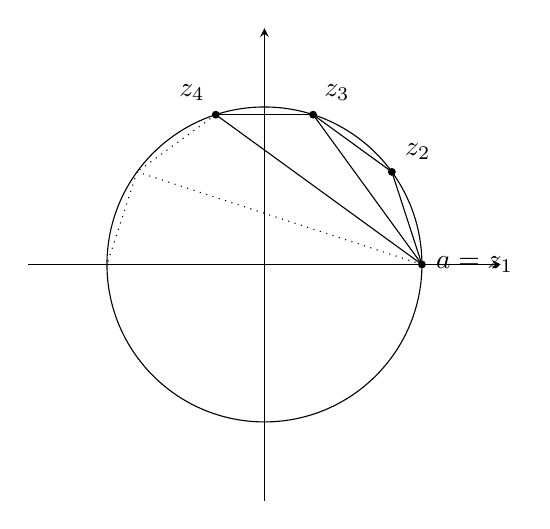
\begin{tikzpicture}
					\tikzset{>=stealth}
					\draw[->] (-3, 0) -- ++(6, 0) coordinate (X);
					\draw[->] (0, -3) -- ++(0, 6);
					\newcommand \CircleRadius {2};
					\newcommand \Vertices {10};
					\draw(0, 0) circle (\CircleRadius);
					\foreach \i [evaluate=\i as \x using (\i - 1)*(360 / \Vertices)] in {1, ..., 6} {
						\coordinate (z\i) at (\x:\CircleRadius);
						\ifthenelse{\i<5}{
							\node[label={\x:{\ifthenelse{\i=1}{$a=z_\i$}{$z_\i$}}},circle,fill,inner sep=1pt] at (z\i) {};
						}{};
					};
					\foreach \i [evaluate=\i as \j using \i + 1] in {1, ..., 5} {
						\ifthenelse{\i<4}{
							\draw (z\i)--(z\j);
						}{
							\draw[dotted] (z\i)--(z\j);
						}
					}
					\draw (z1)--(z3);
					\draw (z1)--(z4);
					\draw[dotted] (z1)--(z5);
				\end{tikzpicture}
			\end{center}
			\caption[loftitle]{A regular $n$-gon with the roots of unity on its vertices}
			\label{figure:regular n-gon with roots of unity}
		\end{figure}

		Thus the equation that we wish to prove becomes
		\begin{equation}\label{eq:total length from one vertex to all others is n}
			\abs{1 - z_2}\abs{1 - z_3}\hdots\abs{1 - z_n} = n
		\end{equation}
		Note that $z_2, ..., z_n$ are the $n$th roots of unity other than 1.

		Let $z$ be a variable and consider the polynomial
		\begin{equation}\label{eq:roots of unity polynomial}
			P(z) := 1 + z + z^2 + \hdots + z^{n - 1}
		\end{equation}
		Since the roots of $P(z)$ are the $n$th roots of unity other than 1, we can factorize \cref{eq:roots of unity polynomial} into
		\begin{equation*}
			P(z) = (z - z_2)(z - z_3) \hdots (z - z_n)
		\end{equation*}
		Now let $z = 1$ and take the modulus of $P(z)$, and we get \cref{eq:total length from one vertex to all others is n}.
	\end{proof}
\end{ex}

\begin{ex}
	Let $n \in \mathbb{N}$. Show that $\sum_{j=0}^{n} \binom{3n}{3j} = \frac{2^{3n} + 2(-1)^n}{3}$.

	\begin{proof}
		Let $\alpha = e^{i \frac{2\pi}{3}}$. Then $\alpha$ is a cubic root of unity, i.e. $\alpha^3 = 1$, and from \cref{ex:sum of root of unity other than one is negative one}, $1 + \alpha + \alpha^2 = 0$.

		Consider
		\begin{align}
			\begin{split}\label{eq:combinatorial problem solved in complex terminology 1}
			(1 + 1)^{3n}
				=& \binom{3n}{0} + \binom{3n}{1} + \binom{3n}{2} + \binom{3n}{3} + \binom{3n}{4} \\
				&+ \binom{3n}{5} + \binom{3n}{6} + \hdots + \binom{3n}{3n}
			\end{split} \\
			\begin{split}\label{eq:combinatorial problem solved in complex terminology 2}
			(1 + \alpha)^{3n}
				=& \binom{3n}{0} + \binom{3n}{1}\alpha + \binom{3n}{2}\alpha^2 + \binom{3n}{3} + \binom{3n}{4}\alpha \\
				&+ \binom{3n}{5}\alpha^2 + \binom{3n}{6} + \hdots + \binom{3n}{3n}
			\end{split} \\
			\begin{split}\label{eq:combinatorial problem solved in complex terminology 3}
			(1 + \alpha^2)^{3n}
				=&\binom{3n}{0} + \binom{3n}{1}\alpha^2 + \binom{3n}{2}\alpha + \binom{3n}{3} + \binom{3n}{4}\alpha^2 \\
				&+ \binom{3n}{5}\alpha + \binom{3n}{6} + \hdots + \binom{3n}{3n}
			\end{split}
			\phantom{a}
		\end{align}

		Adding \cref{eq:combinatorial problem solved in complex terminology 1}, \cref{eq:combinatorial problem solved in complex terminology 2} and \cref{eq:combinatorial problem solved in complex terminology 3}, we observe that the terms with coefficients $\binom{3n}{k}$ where $k$ is not a multiple of 3 sums to 0 as given by $1 + \alpha + \alpha^2 = 0$, and therefore we obtain
		\begin{align*}
			2^{3n} + (1 + \alpha)^{3n} + (1 + \alpha^2)^{3n} &= 3 \sum_{j=0}^{n} \binom{3n}{3j} \\
			\frac{1}{3} \left[2^{3n} + (1 + \alpha)^{3n} + (1 + \alpha^2)^{3n}\right] &= \sum_{j=0}^{n} \binom{3n}{3j} \\
			\frac{1}{3} \left[2^{3n} + (-\alpha^2)^{3n} + (-\alpha)^{3n} \right] &= \sum_{j=0}^{n} \binom{3n}{3j} \quad \text{since } 1 + \alpha + \alpha^2 = 0 \\
			\frac{1}{3} \left[2^{3n} + (-1)^n + (-1)^n \right] &= \sum_{j=0}^{n} \binom{3n}{3j} \quad \text{since } \alpha^3 = 1 \\
			\frac{2^{3n} + 2(-1)^n}{3} &= \sum_{j=0}^{n} \binom{3n}{3j}
		\end{align*}
		as required.
	\end{proof}
\end{ex}

\begin{ex}
	Note that we can define $\Arg{z}$ in any interval of length $2 \pi$, i.e. it is not necessary that $\Arg{z} \in [0, 2\pi)$.

	For example, if we restrict $\Arg{z} \in [-\pi, \pi]$, then we can write
	\begin{equation*}
		\Arg{\left(-\frac{1}{\sqrt{2}} - \frac{1}{\sqrt{2}} i \right)} = - \frac{3\pi}{4}
	\end{equation*}

	Let $z$ be on the unit circle and $\Arg{z} \in [-\pi, \pi]$. Suppose that $z \notin \mathbb{R}$, i.e. $z \neq 1, z \neq -1$. Show that
	\begin{equation*}
		\Arg{\left( \frac{z-1}{z+1} \right)} = \begin{cases}
			\frac{\pi}{2} & \im{z} > 0 \\
			-\frac{\pi}{2} & \im{z} < 0
		\end{cases}
	\end{equation*}

	\begin{proof}
		Note that $\forall w_1, w_2 \in \mathbb{C}$, where $\Arg{w_1} = \tau_1, \Arg{w_2} = \tau_2$ for $\tau_1, \tau_2$ in the same $2\pi$-interval,
		\begin{equation*}
			\Arg{\frac{w_1}{w_2} = \frac{e^{i\tau_1}}{e^{i\tau_2}} \equiv e^{i (\tau_1 - \tau_2)} = \Arg{w_1} - \Arg{w_2}}
		\end{equation*}
		in modulo $2\pi$.

		Suppose $\im{z} > 0$. Let $\theta_1 = \Arg{(z - 1)}$ and $\theta_2 = \Arg{(z + 1)}$. Consider \cref{figure:angle division example}. We observe that
		\begin{align*}
			\frac{\pi}{2} &= \theta_2 + \pi - \theta_1 \\
			\theta_1 - \theta_2 &= \frac{\pi}{2}
		\end{align*}
		as desired.

		\begin{figure}
			\begin{center}
				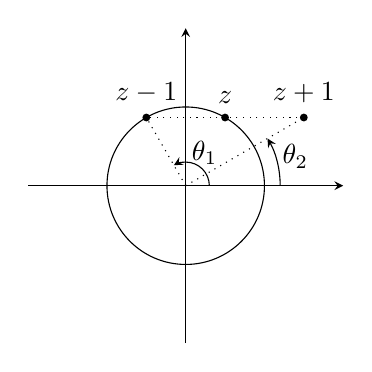
\begin{tikzpicture}
					\tikzset{>=stealth}
					\draw[->] (-2, 0) -- ++(4, 0) coordinate (X);
					\draw[->] (0, -2) -- ++(0, 4);
					\coordinate (O) at (0,0);
					\draw (0,0) circle (1);
					\coordinate (z) at (60:1);
					\node[label={90:{$z$}},circle,fill,inner sep=1pt] at (z) {};
					\coordinate (z-1) at ($(z) + (-1,0)$);
					\node[label={90:{$z-1$}},circle,fill,inner sep=1pt] at (z-1) {};
					\coordinate (z+1) at ($(z) + (1,0)$);
					\node[label={90:{$z+1$}},circle,fill,inner sep=1pt] at (z+1) {};
					\draw[dotted] (z+1)--(z-1);
					\draw[dotted] (O)--(z-1);
					\draw[dotted] (O)--(z+1);
					\path (X) -- (O) -- (z-1) pic [draw,->,pic text=$\theta_1$, angle radius=0.3cm,angle eccentricity=1.6] {angle=X--O--z-1};
					\path (X) -- (O) -- (z+1) pic [draw,->,pic text=$\theta_2$, angle radius=1.2cm,angle eccentricity=1.2] {angle=X--O--z+1};
				\end{tikzpicture}
				\hspace{3cm}
				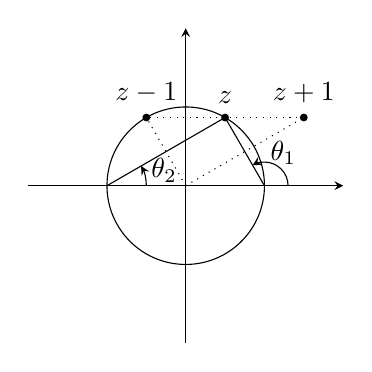
\begin{tikzpicture}
					\tikzset{>=stealth}
					\draw[->] (-2, 0) -- ++(4, 0) coordinate (X);
					\draw[->] (0, -2) -- ++(0, 4);
					\coordinate (O) at (0,0);
					\draw (0,0) circle (1);
					\coordinate (z) at (60:1);
					\node[label={90:{$z$}},circle,fill,inner sep=1pt] at (z) {};
					\coordinate (z-1) at ($(z) + (-1,0)$);
					\node[label={90:{$z-1$}},circle,fill,inner sep=1pt] at (z-1) {};
					\coordinate (z+1) at ($(z) + (1,0)$);
					\node[label={90:{$z+1$}},circle,fill,inner sep=1pt] at (z+1) {};
					\coordinate (-1) at (180:1);
					\coordinate (1) at (0:1);
					\draw[dotted] (z+1)--(z-1);
					\draw[dotted] (O)--(z-1);
					\draw[dotted] (O)--(z+1);
					\draw (-1)--(z);
					\draw (1)--(z);
					\path (X)--(-1)--(z) pic[draw,->,pic text=$\theta_2$,angle eccentricity=1.5] {angle=X---1--z};
					\path (X)--(1)--(z) pic[draw,->,pic text=$\theta_1$,angle radius=0.3cm,angle eccentricity=1.6] {angle=X--1--z};
				\end{tikzpicture}
			\end{center}
			\caption[loftitle]{(Right) Depicted question, (Left) Translated Angles}
			\label{figure:angle division example}
		\end{figure}

		Similarly, we can obtain $\theta_1 - \theta_2 = -\frac{\pi}{2}$ for when $\im{z} < 0$. This completes the proof.
	\end{proof}
\end{ex}

\begin{ex}
	Let $f(z) = e^z$ for $z \in \mathbb{C}$. Let $A = \{z = x + iy \in \mathbb{C} : x \leq 1, y \in [0, \pi] \}$. Describe the image of $f(A)$.

	\begin{solution}
		Firstly, note that
		\begin{align*}
			e^z &= e^{x + iy} \\
			e^x &\in (0, e] \\
			y &\in [0, \pi]
		\end{align*}
		It is clear that the image will be in on the positive side of the imaginary-axis. Also, since $e^x \in (0, e]$, we get the right graph represented in \cref{figure:domain and image of f(A)}. The image of $f(A)$ is described in the left image of \cref{figure:domain and image of f(A)}.

		\begin{figure}
			\begin{center}
				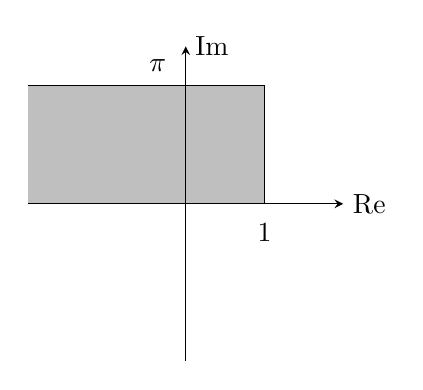
\begin{tikzpicture}
					\tikzset{>=stealth}
					\draw[->] (-2, 0) -- ++(4, 0) coordinate (X) node[below, right] {$\re$};
					\draw[->] (0, -2) -- ++(0, 4) node[above,right] {$\im$};
					\draw [draw=none,fill=black,fill opacity=0.25] (-2,0) rectangle (1,1.5);
					\draw (1,0)--(1,1.5)--(-2,1.5);
					\node[label={270:{$1$}}] at (1,0) {};
					\node[label={155:{$\pi$}}] at (0,1.5) {};
				\end{tikzpicture}
				\hspace{3cm}
				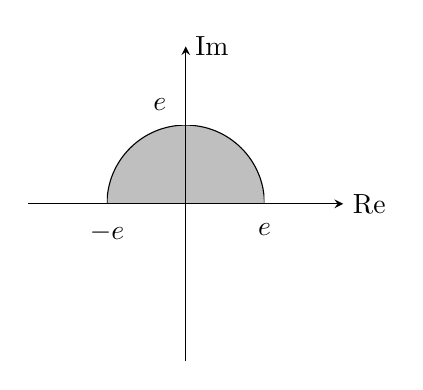
\begin{tikzpicture}
					\tikzset{>=stealth}
					\draw[->] (-2, 0) -- ++(4, 0) coordinate (X) node[below,right] {$\re$};
					\draw[->] (0, -2) -- ++(0, 4) node[above,right] {$\im$};
					\begin{scope}
					    \clip (-1,0) rectangle (1,1);
					    \draw[fill=black,fill opacity=0.25] (0,0) circle(1);
					    \draw (-1,0) -- (1,0);
					\end{scope}
					\node[label={270:{$e$}}] at (1,0) {};
					\node[label={270:{$-e$}}] at (-1,0) {};
					\node[label={155:{$e$}}] at (0,1) {};
				\end{tikzpicture}
			\end{center}
			\caption[loftitle]{(Right) Domain of $f(A)$, (Left) Image of $f(A)$}
			\label{figure:domain and image of f(A)}
		\end{figure}
	\end{solution}
\end{ex}

\end{document}